\documentclass[t]{beamer}
\usetheme{Madrid}
\usecolortheme{default}

\usepackage{booktabs} % Untuk garis \toprule, \midrule, \bottomrule
\usepackage{graphicx} % Untuk \resizebox
\usepackage{tikz}
\usetikzlibrary{trees}


\title[Visualisasi Data - Pertemuan 1]{Why: Task Abstraction?}

\author{Ahmad Luky Ramdani}
\subtitle{Matakuliah Visualisasi Data (Data visualization)}
\author[Ahmad Luky Ramdani]{Ahmad Luky Ramdani \and Ira Safitri \and Dimas Dwi Randa}
\institute[ITERA]
{
  Program Studi Data Sains\\
  Fakultas Sains \\
  Institut Teknologi Sumatera
}

\date{Bandung, \today}
\begin{document}



\frame{\titlepage}


% ------------------------------
\begin{frame}{Why: Task Abstraction?}
    \begin{block}{Tujuan Pembelajaran}
        Mampu mengabstraksi tugas dari domain spesifik menjadi kosakata umum (\textit{Action} \& \textit{Target}) untuk menentukan solusi visual yang tepat.
    \end{block}

    \vspace{0.4cm}
    \textbf{Topik Pembahasan Utama:}
    \begin{enumerate}
        \item \textbf{High-level Actions:} Mengonsumsi vs Memproduksi data.
        \item \textbf{Search Levels:} Strategi mencari berdasarkan pengetahuan lokasi dan target.
        \item \textbf{Query Levels:} Tingkat kedalaman pertanyaan (Identifikasi $\rightarrow$ Komparasi $\rightarrow$ Ringkasan).
        \item \textbf{Targets:} Fokus analisis pada tren, outlier, atau fitur spesifik dataset.
    \end{enumerate}
\end{frame}

% ------------------------------


\begin{frame}{Why: Task Abstraction?}
    \vspace{-0.3cm}
    \begin{block}{Task Abstraction}
        	Tentang memahami niat di balik sebuah visualisasi. Jika pertemuan sebelumnya bertanya "Data apa yang kita punya?", maka saat ini bertanya "Apa yang ingin dicapai pengguna dengan data tersebut?".
    \end{block}
    \vspace{-0.3cm}
    \begin{center}
    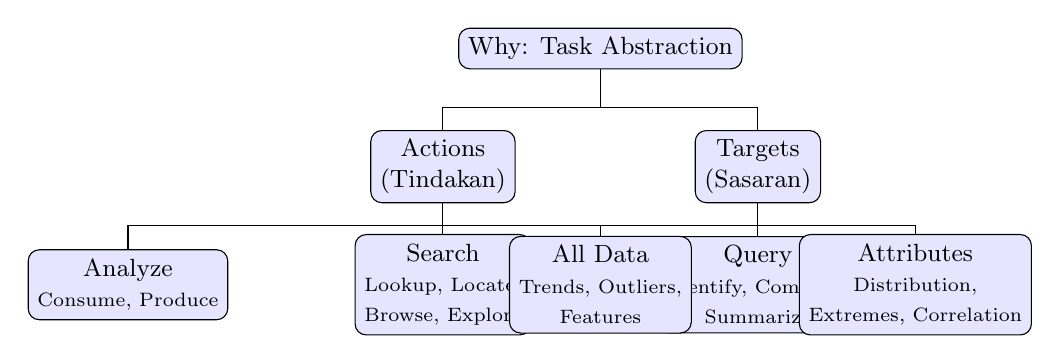
\begin{tikzpicture}[edge from parent fork down, sibling distance=4cm, level distance=1.5cm, every node/.style={fill=blue!10, rounded corners, draw, align=center, font=\small}]
        \node {Why: Task Abstraction}
            child {node {Actions \\ (Tindakan)}
                child {node {Analyze \\ \scriptsize Consume, Produce}}
                child {node {Search \\ \scriptsize Lookup, Locate, \\ \scriptsize Browse, Explore}}
                child {node {Query \\ \scriptsize Identify, Compare, \\ \scriptsize Summarize}}
            }
            child {node {Targets \\ (Sasaran)}
                child {node {All Data \\ \scriptsize Trends, Outliers, \\ \scriptsize Features}}
                child {node {Attributes \\ \scriptsize Distribution, \\ \scriptsize Extremes, Correlation}}
            };
    \end{tikzpicture}
    \end{center}
    \centering \textit{"Abstraksi tugas memungkinkan kita merancang visualisasi yang berfokus pada tujuan pengguna, bukan hanya pada ketersediaan data."}

   
\end{frame}

% ------------------------------


\begin{frame}{Why: Task Abstraction?}
    \begin{block}{Task Abstraction}
        
    \end{block}
   
\end{frame}


% --- Final page ---
\begin{frame}[c]
    \centering
    \Huge{Terima Kasih} % 
    
    \vspace{1.5cm}
    \normalsize
    \textbf{Ahmad Luky Ramdani} \\ % 
    \href{mailto:ahmadluky@sd.itera.ac.id}{ahmadluky@sd.itera.ac.id} % 
\end{frame}

\end{document}
